\documentclass{article}
\usepackage{tikz}
\usetikzlibrary{arrows.meta,positioning,calc,shapes.geometric}
\pagestyle{empty}
\begin{document}
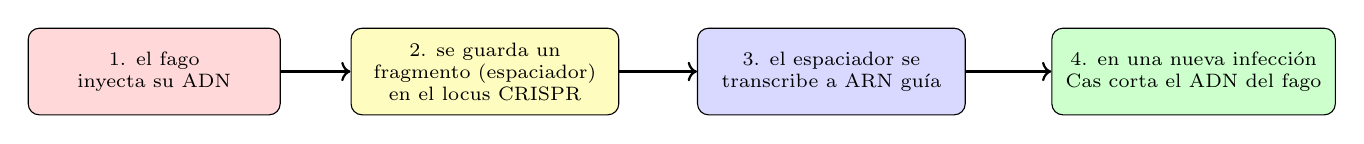
\begin{tikzpicture}
\tikzset{every node/.append style={align=center}}

\def\bx#1#2#3{\node[draw, rounded corners, fill=#3, minimum width=3.0cm, minimum height=1.0cm, align=center, font=\scriptsize] (#1) at (#2) {};}
\node[draw, rounded corners, fill=red!15, minimum width=3.2cm, minimum height=1.1cm, align=center, font=\scriptsize] (a) at (0,0) {1. el fago\\ inyecta su ADN};
\node[draw, rounded corners, fill=yellow!25, minimum width=3.4cm, minimum height=1.1cm, align=center, font=\scriptsize] (b) at (4.2,0) {2. se guarda un\\ fragmento (espaciador)\\ en el locus CRISPR};
\node[draw, rounded corners, fill=blue!15, minimum width=3.4cm, minimum height=1.1cm, align=center, font=\scriptsize] (c) at (8.6,0) {3. el espaciador se\\ transcribe a ARN guía};
\node[draw, rounded corners, fill=green!20, minimum width=3.6cm, minimum height=1.1cm, align=center, font=\scriptsize] (d) at (13.2,0) {4. en una nueva infección\\ Cas corta el ADN del fago};
\draw[->, thick] (a) -- (b); \draw[->, thick] (b) -- (c); \draw[->, thick] (c) -- (d);

\end{tikzpicture}
\end{document}
